\documentclass[a4paper]{article}
\usepackage[english]{babel}
\usepackage{multicol}
\usepackage{amsmath}
\usepackage{amsfonts}
\usepackage{amssymb}
\usepackage[font=scriptsize]{caption}
\usepackage{parskip}
\usepackage[a4paper, margin=1in, total={6in, 8in}]{geometry}
\usepackage{titling}
\usepackage{subcaption}
\usepackage{float}
\usepackage{placeins}
\usepackage{graphicx}

\parskip = 6pt plus 2pt minus 2pt
\setlength{\droptitle}{-2cm}

\title{HW6 - Computer Simulation II}
\author{Schewtschik, Guilherme (3748052)}
\date{\today}

\begin{document}
\maketitle
\section{}
Generalizing the wolff algorithm to the XY model we can measure the mean energy per site, specific heat, and susceptibility for: $\beta \in [0,2]$ in steps of $0.05$ for $8\times 8$ and $24\times 24$ lattices

\begin{figure}[H]
    \centering
    \begin{minipage}{0.48\linewidth}
        \centering
        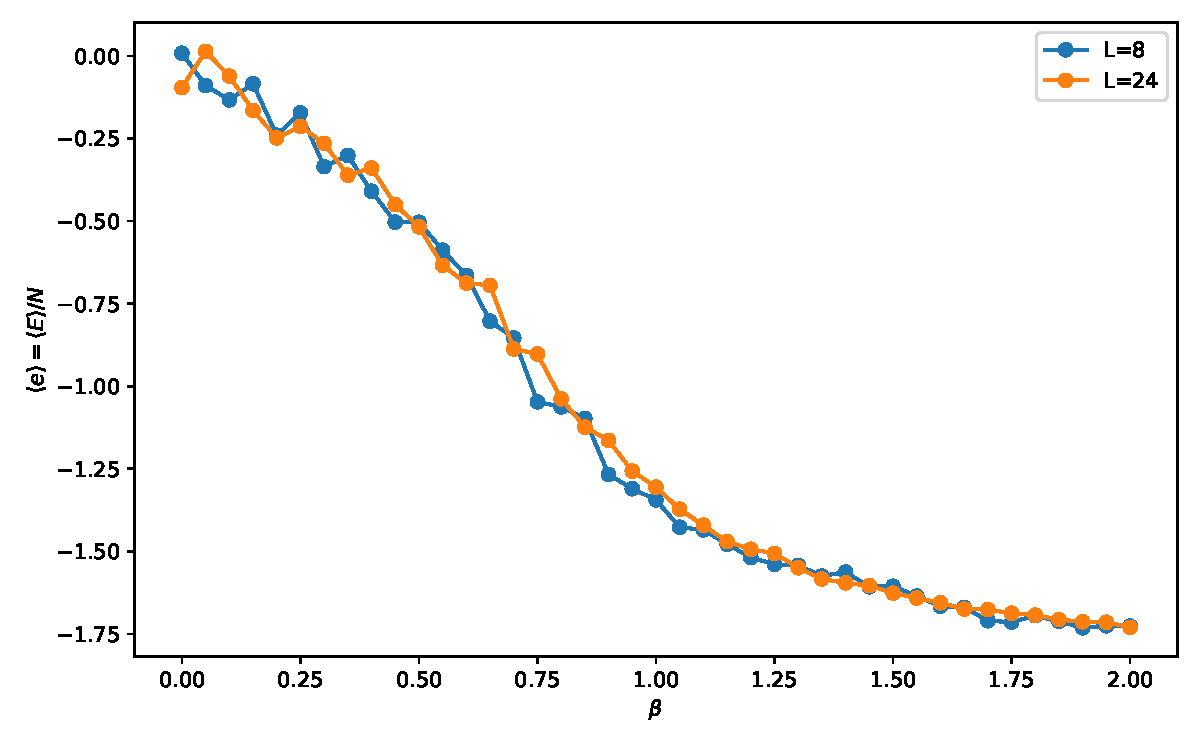
\includegraphics[width=\linewidth]{figures/xy_energy_vs_beta1.pdf}
        \caption{Mean energy per site x $\beta$.}
    \end{minipage}
    \hfill
    \begin{minipage}{0.48\linewidth}
        \centering
        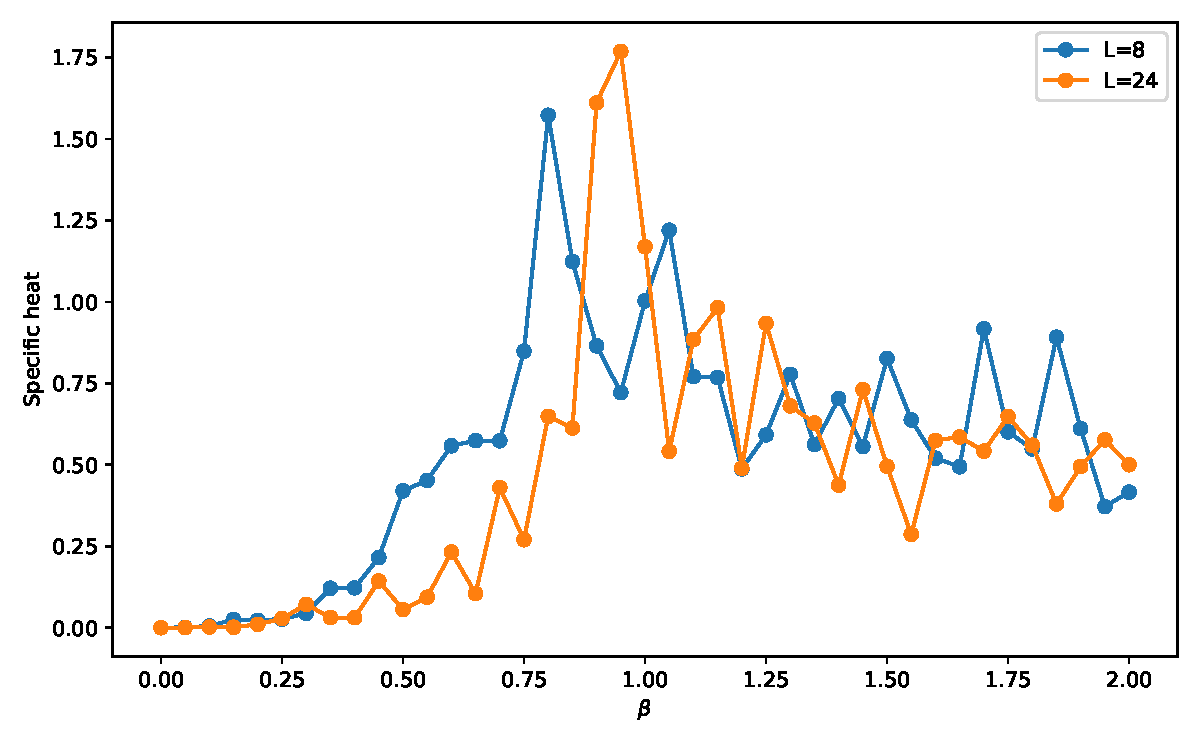
\includegraphics[width=\linewidth]{figures/xy_specific_heat_vs_beta1.pdf}
        \caption{Specific heat x $\beta$.}
    \end{minipage}
\end{figure}

\begin{figure}[H]
    \centering
    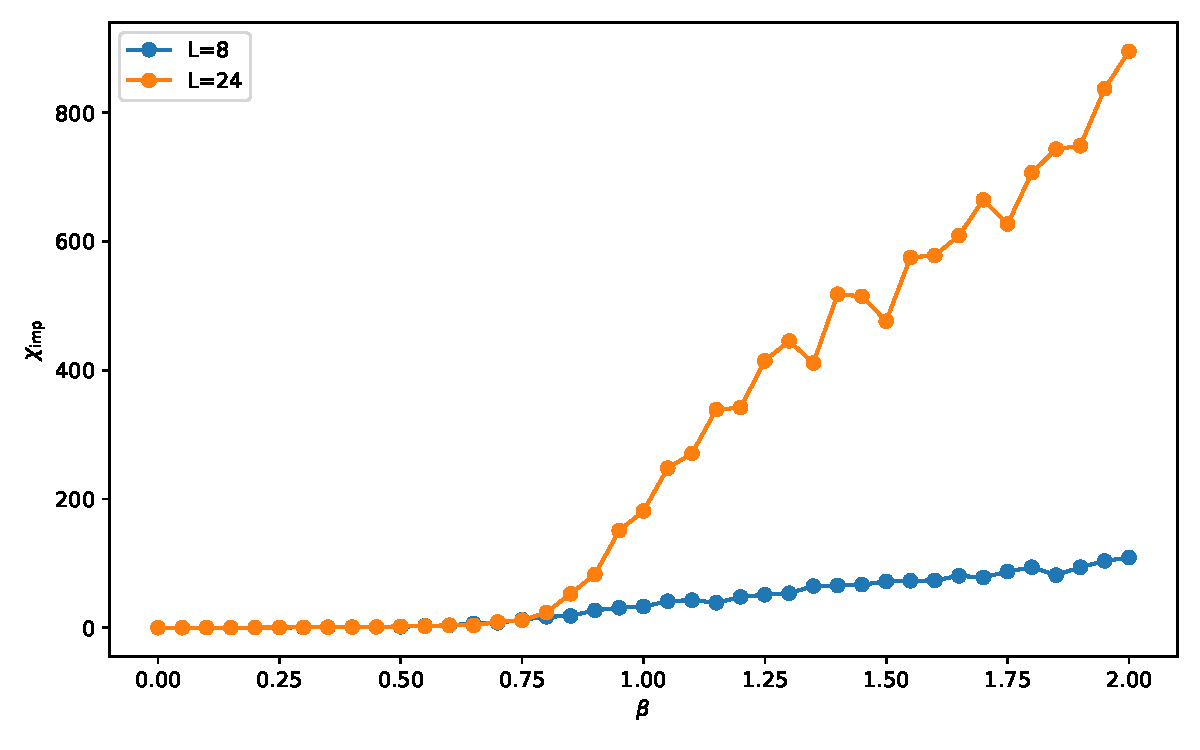
\includegraphics[width=0.7\linewidth]{figures/xy_susceptibility_vs_beta1.pdf}
    \caption{susceptibility x $\beta$.}
\end{figure}

We can see the energy per site decreases with $\beta$ (as expected) for both lattice sizes, the specific heat peaks around $\beta = 1$,
and the susceptibility increases with $\beta$, showing a more pronounced increase around $\beta = 1$ for the larger lattice, indicating critical behavior.  
\newpage
\section{}
For the $24\times 24$ lattice, we compared the standard and improved susceptibility estimators at $\beta = 1.0$, $0.9$, $0.8$, $0.7$, $0.6$, and $0.5$.

\begin{figure}[H]
    \centering
    \begin{minipage}{0.48\linewidth}
        \centering
        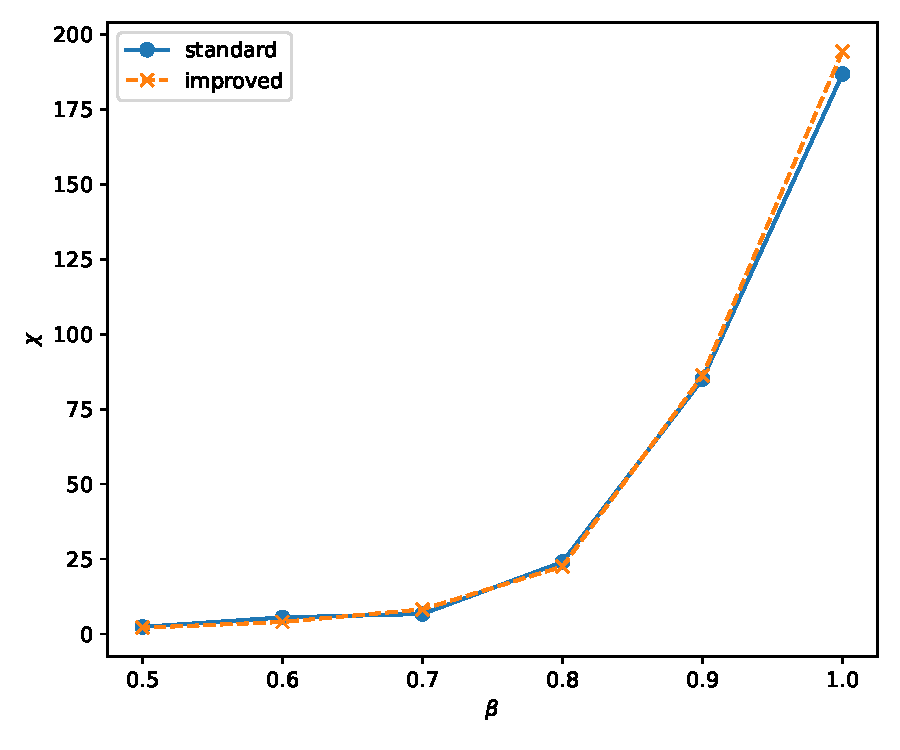
\includegraphics[width=\linewidth]{figures/xy_high_temp_susceptibility_comparison1.pdf}
        \caption{Standard x improved susceptibility.}
    \end{minipage}
    \hfill
    \begin{minipage}{0.48\linewidth}
        \centering
        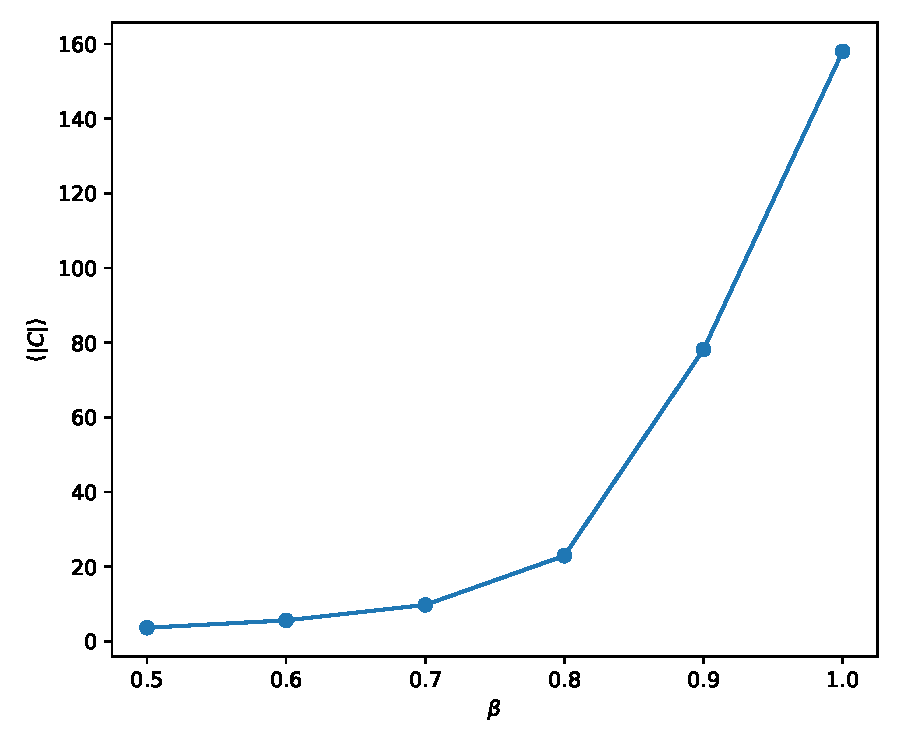
\includegraphics[width=\linewidth]{figures/xy_high_temp_cluster_size1.pdf}
        \caption{Mean cluster size at the comparison points.}
    \end{minipage}
\end{figure}

\begin{figure}[H]
    \centering
    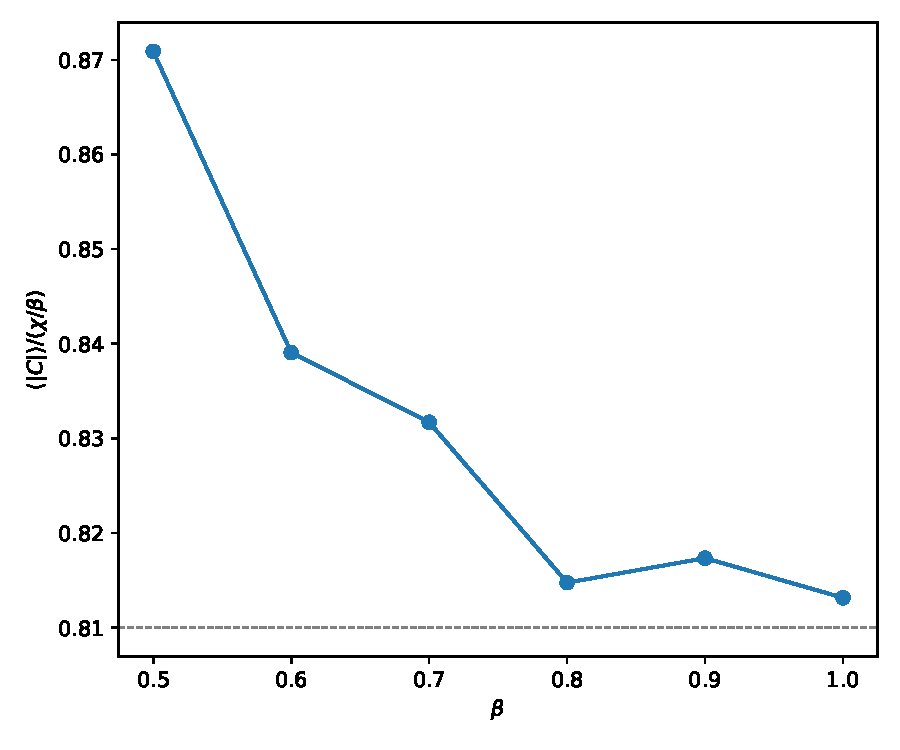
\includegraphics[width=0.7\linewidth]{figures/xy_high_temp_cluster_ratio1.pdf}
    \caption{Ratio of mean cluster size to the improved susceptibility.}
\end{figure}


The improved susceptibility estimator remains close to the standard estimator being only slightly higher for bigger $\beta$ values,
the mean cluster size increases rapidly with $\beta$, and the ratio between the mean cluster size and the susceptibility 
remains above the expected $0.81$, for small $\beta$ values ranging from $0.87$ to $0.82$ only really approaching the expected value for smaller $\beta$,
 due to the bigger correlation lenghts.
\end{document}
